まったく、
この話をするのも何度目だろうかという話で、
私としても、持ち前のサービス精神を発揮して、
話す度に違う切り口で以ってして毎度新鮮な印象をもたせようとしたし、
それはそれで、
皆さんにはそれなりに楽しんでもらえてたようである.
時としてはつい、
(これはあくまでも観客を飽き飽きさせまいと苦心する私のサービス精神ゆえであるが、)
事実とはまるで違う結論で終えたり、
突拍子もないイベントを勝手に挿入しすぎたせいで、物語の辻褄が合わなくなり、
結局結論までたどり着かなかったりもした.
しかし今回は、楽しませることを目的とするよりは、
文字で記録することを一番の目的とするようだから、
あくまでも出来事を観測した順番通りに、見たままを正確に記録していくことにしよう.
となると、語りはまたここから始めなければならないことになる.
まったく、なんと面倒くさい.

\subsection*{駅前にて}

その土地の形を、よく見知ったと期待される物の形に例えることで説明をしてみようかと思ったが、
いくつかの理由でこれは不採用にする.
一番の理由は、書いてる側も呼んでる側も気恥ずかしさを負うことにある.
これ以上の説明は要らないだろう.
だからもう、私はありのままを丁寧に説明するだけにしよう.

\begin{wrapfigure}{r}{0.5\textwidth}
  \hspace*{-.1\textwidth}
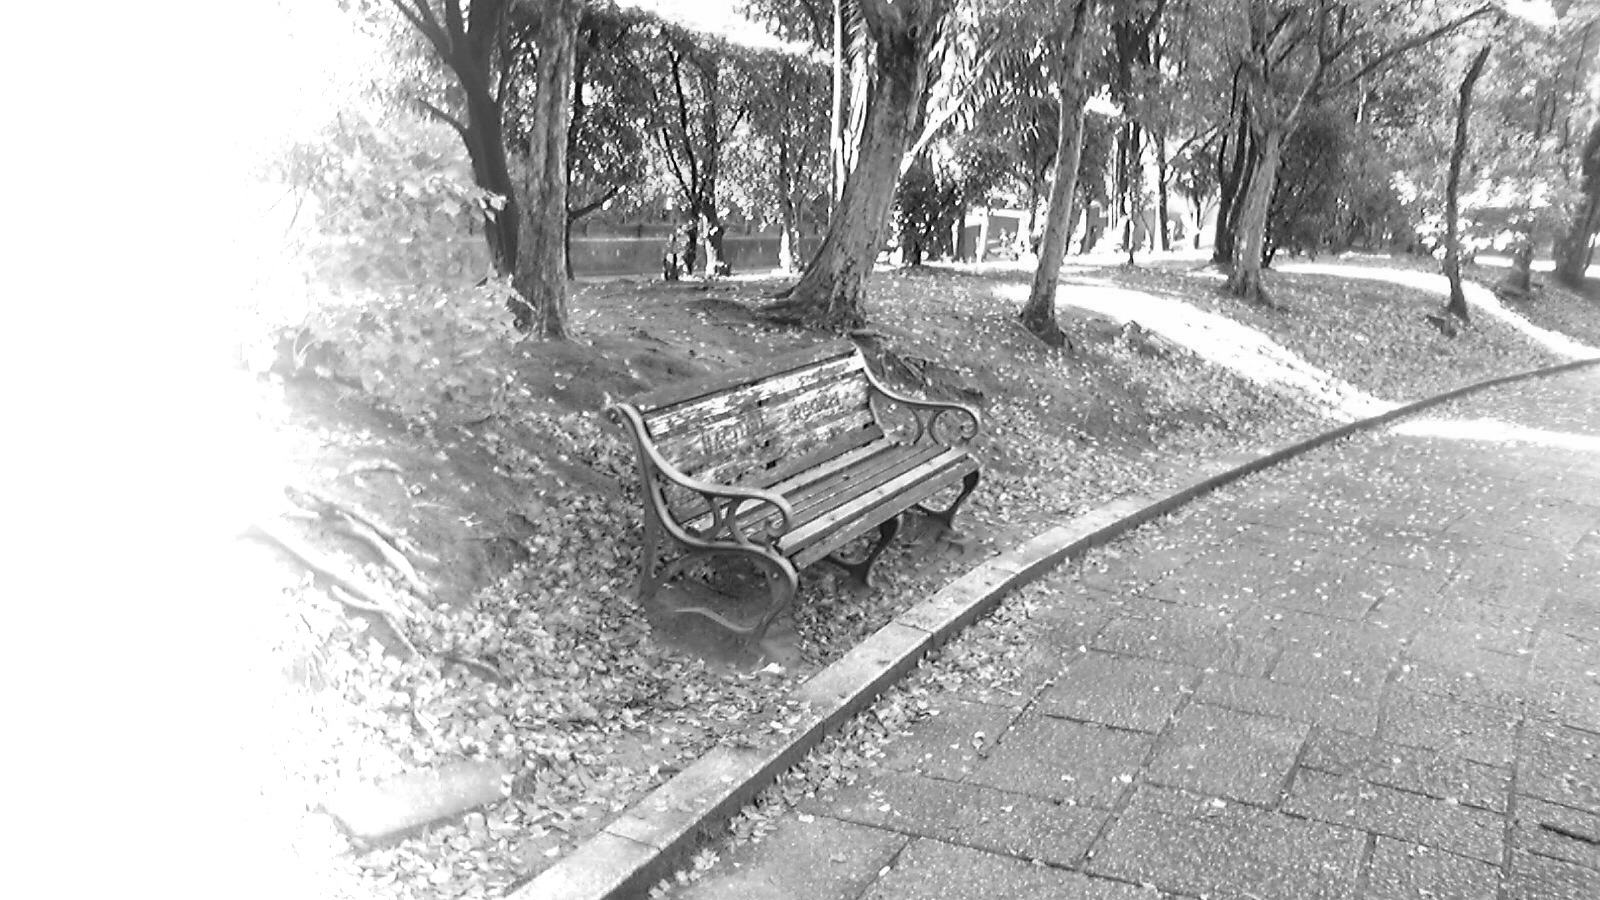
\includegraphics[width=0.58\textwidth,bb=0 0 1600 900]{img/park1.jpg}
\end{wrapfigure}

駅というのは普通、街の中心にあるものだ.
それは普通、駅を中心に街というのは発展するものだから.
だから駅より北方面、あるいは西側を私が知らないというのはいささか不思議である.
もちろん、いつもいつも、駅が街の中心というわけではない.
私が高校に通うのに使っていた岡本駅は、言ってしまえば六甲山の裾にあって、
駅より北には山しか無い.
というか駅が位置するその場所も、綺麗に舗装されてかなり気づきにくくはなっているものの、
山である.
まだ、山である、と言ったほうが正確か.
つまり、山というからには、山頂から地面は低い方低い方へと走っており、
その勢いは駅を通りすぎてもまだ止まらない.
駅から飛び出た人は、その安定したエネルギーを求めて、自然と足が南に向いてしまうという仕組みになっているのだ.
従って、この駅の場合、駅よりも南しか発展しない.
コンビニも雑貨屋もアイスクリーム屋も、南側にしか存在しない.

対して、この駅は、別になんということはない.
平地の上のぽんとあるだけである.
5分ほど東に歩いてみると大きな坂があって、実は高台にあったのだと気付くが、
しかし、
駅周辺だけを取り出してみれば、別段ただの平地である.
線路はほぼ東西に平行に走っており、
南側の駅口から入るとまず地下におり、そうして線路をくぐったのち、ホームに出る.
それよりも北側に何があるかなんてのは、
ホームから眺めれば分かることで、
なあんにもないのである.
この街に面白さを求めてはいけない.

一応、楽しいことといえば、
駅より10分ほど南に歩くと、割に大きな公園があって、
私は昼休みのほとんどをそこで過ごすのだが、
これはそんなに重要でないので省くことにする.

\subsubsection*{わたしについて}

つまり、線路というのは、強く境界線として働くのだな.
駅が出来て、それから駅を中心に街が発展する場合、
当然線路というものが街の発展に影響を及ぼすだろう.
それがなんだか、線路という結界が街にかけられた呪いみたいで面白くて、
私はメモ帳に
「線路は境界線として強く働く」
とだけ書いてご機嫌だった.
これが私であった.
携帯電話は持たされず、
自分のことを天才だと信じ、
公園でホームレスに話しかけるのがささやかな遊戯で、
得意科目は理数系、
苦手科目は暗記全般.

\hline

私は一人で駅を南口から入り、一旦地下を歩いて、
(小さな駅には似つかわしくないことに地下は二階分の深さがあり、
いつでも30秒で出来たてのハンバーガーを売るお店があり、
個人営業の本屋があり、
その向かいには雀荘があって、
他にも、あんまり注目がしたことがないので何なのかはよく知らないけど、
たぶん、普通に営業するお店が、こんな狭い面積に密集している)
一人で階段でホームにあがる.
一人で電車に乗った.
電車から外の風景を見下ろしていれば、すぐに私の家の最寄り駅に着く.

見下ろすっていうのは、今の場合、まったく適切な表現で、
この線はここから3駅の間、すこし高いところを走る.
下は、長い下り坂になっているが、線路はなお水平に走るためである.

一人の少女が歩いてるのを見た. そして私は、
「彼女はどうして一人なのだろう」 という議論を始めた.
「つまり、彼女は私と同じなんだ」 という説を支持することにした.

\section*{\texttt{(call/cc}}
坂を下る少女が私と同じだと考えた途端、 彼女のことをかわいそうに思えた
(N.B. かわいそうな人であることに気がついた).

それはつまり、私は私のことをかわいそうなの?
という疑念は切って捨てなければならない、と自分に言い聞かせた.
他人だからこそ、かわいそうなのだ. 自己憐憫はもっとかわいそうだ.
自分をかわいそうと思うのは世界で一番かわいそうな人だけの権利でしょう.
自己憐憫は一種の快楽だ. 全く何も産まない、非生産的な快楽だ.
そんなことは、ちょっと頭を掠ったところで、五秒で止めるべきだわ.
そんな人はわざと自分で自分を貶める.
それでそんな状況を誰かにひけらかしたがる.
凛々しい猫よりも、濡れて泥に汚れたしょぼくれた猫のほうが大切に扱われると信じてる.
そんな姿、見せることを恥だと思わない. 見せられた方はたまらないと思う.
ああ、つまらないことを考えた. ようするに、ね.
私は可哀想ではないから、もっと下を見るのだ.
言い換えればもっとかわいそうな人がどこかにいるのだ.
例えば、そこにいる、 可哀想な少女は、地面にしゃがみこんでいて、
そうして、私と彼女との距離はまもなく見えないほど離れていった.
まったく可愛そうだ!

\section*{\texttt{(lambda (k)}}

トンネルが間もなく近づくと、
私は習慣として、カバンから煮干しチップの小袋を一つ取り出し、
一口だけつまんで食べた.
ここのトンネルは車専用となっており、
歩行者と自転車は、一つ遠回りをしないといけない.
ちょうどその周辺は野良猫が巣窟になっている.
私がその道路に出ると、彼女たちの半分が四方八方に散る.
それでも残るのはまだ小さな子猫たちだ.
逆に言えば、人間を見て逃げるような猫というのは大きな大人に限るので、
「蜘蛛の子を散らす」という表現は使いにくい.
それにしても、
この世界において、野良猫に天敵もなにもないだろうに、
どうして人間を嫌うのかしら.
私は一匹の子猫のそばでしゃがみこんで、
手に持っていた小袋から煮干を一つつまんでみせた.
子猫たちは、それよりはお腹を撫でて欲しいようなんだな、これが.

\begin{wrapfigure}{r}{0.6\textwidth}
  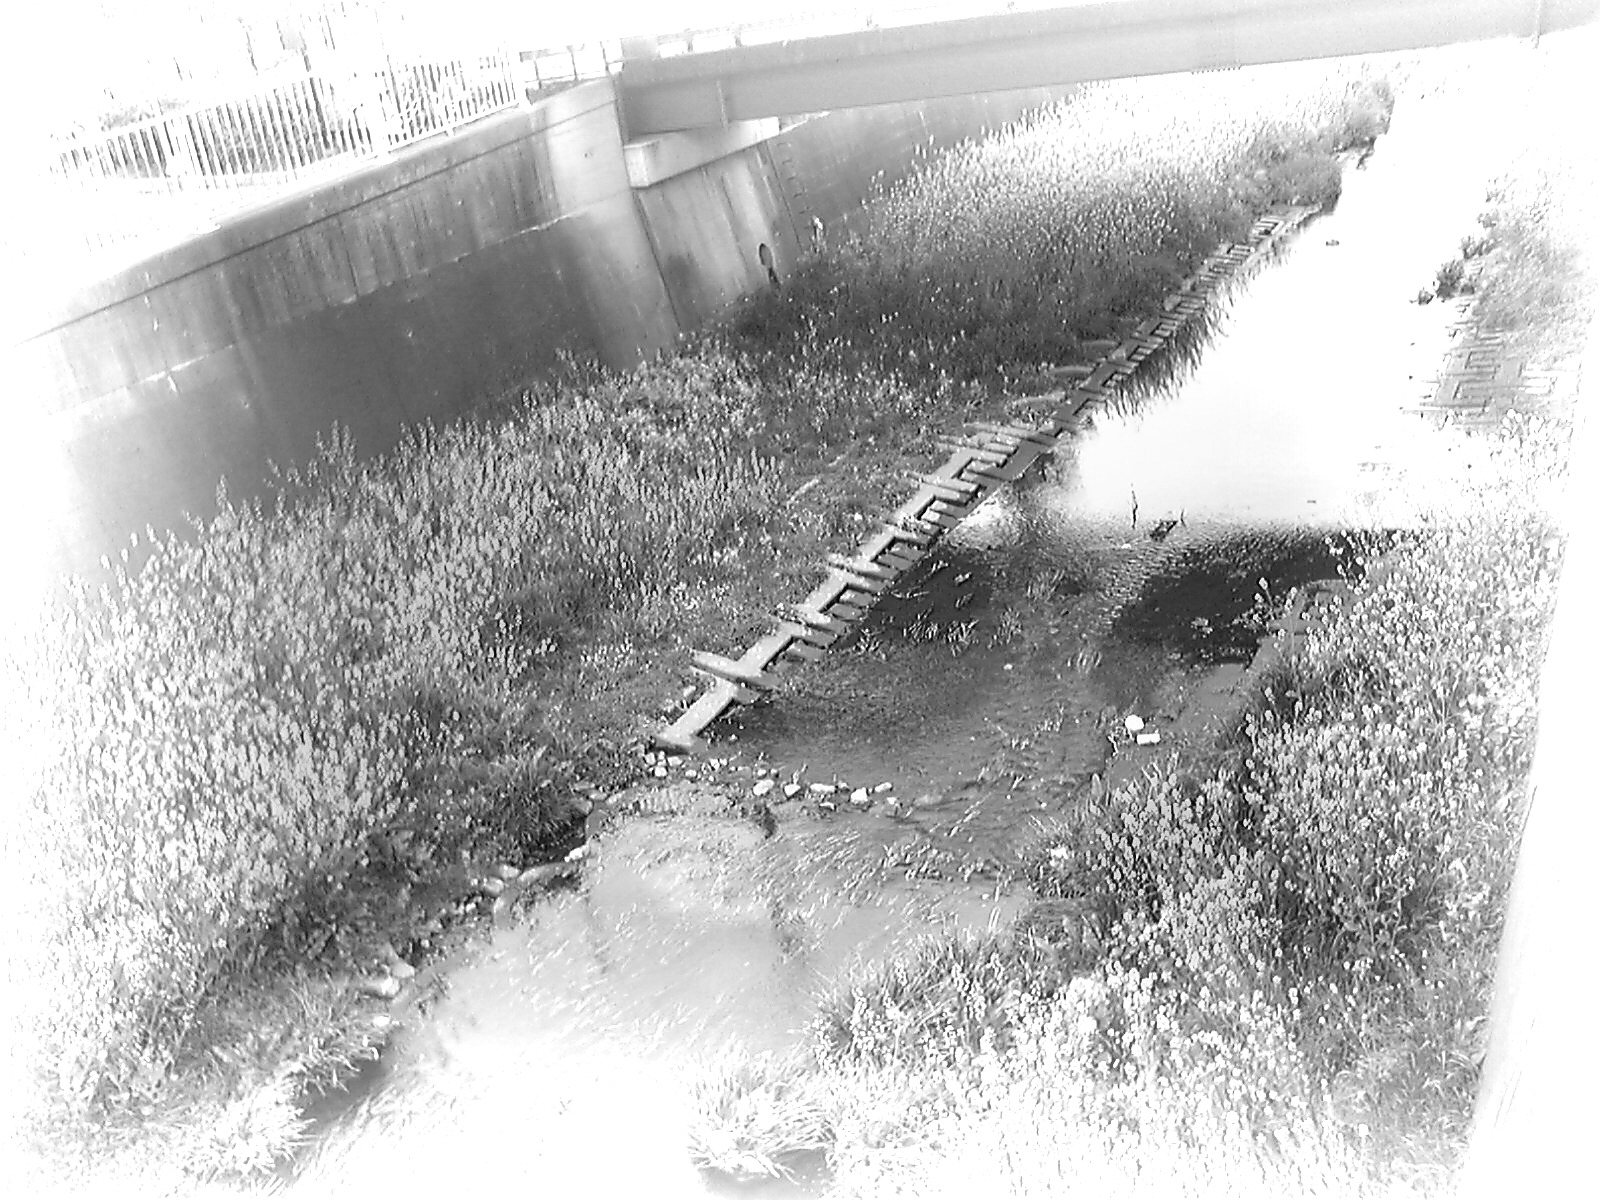
\includegraphics[width=0.58\textwidth,bb=0 0 1600 1200]{img/river.jpg}
\end{wrapfigure}

私が子猫に餌付けする様子を少し遠くから伺う大人たち、
歩行者用のトンネルの裏側の落書き、
川に投げ捨てられて錆びついた自転車、
それくらいのもので、どれも全く毎日見てきたものだ.

象の卵はあれだぞう 象の卵はあれだぞう 象の卵はあれだぞう 象の卵はあれだぞう 象の卵はあれだぞう
象の卵はあれだぞう 象の卵はあれだぞう 象の卵はあれだぞう 象の卵はあれだぞう 象の卵はあれだぞう
象の卵はあれだぞう 象の卵はあれだぞう 象の卵はあれだぞう 象の卵はあれだぞう 象の卵はあれだぞう
象の卵はあれだぞう 象の卵はあれだぞう 象の卵はあれだぞう 象の卵はあれだぞう 象の卵はあれだぞう
象の卵はあれだぞう 象の卵はあれだぞう 象の卵はあれだぞう 象の卵はあれだぞう 象の卵はあれだぞう
象の卵はあれだぞう 象の卵はあれだぞう 象の卵はあれだぞう 象の卵はあれだぞう 象の卵はあれだぞう
象の卵はあれだぞう 象の卵はあれだぞう 象の卵はあれだぞう 象の卵はあれだぞう 象の卵はあれだぞう
象の卵はあれだぞう 象の卵はあれだぞう 象の卵はあれだぞう 象の卵はあれだぞう 象の卵はあれだぞう
象の卵はあれだぞう 象の卵はあれだぞう 象の卵はあれだぞう 象の卵はあれだぞう 象の卵はあれだぞう
象の卵はあれだぞう 象の卵はあれだぞう 象の卵はあれだぞう 象の卵はあれだぞう 象の卵はあれだぞう
象の卵はあれだぞう 象の卵はあれだぞう 象の卵はあれだぞう 象の卵はあれだぞう 象の卵はあれだぞう
象の卵はあれだぞう 象の卵はあれだぞう 象の卵はあれだぞう 象の卵はあれだぞう 象の卵はあれだぞう
象の卵はあれだぞう 象の卵はあれだぞう 象の卵はあれだぞう 象の卵はあれだぞう 象の卵はあれだぞう
